\section{Выполнение работы}
\subsection{Описание предметной области}
В лаборатории работают ученые (scientists),
у ученого есть имя, зарплата.

Ученые разрабатывают животных (creatures).
У животных есть название, время создания, размер.
Животное может иметь несколько создателей.

Животные находятся в клетках.
У клеток есть размер, материал.
Одно животное может находиться в одной клетке.

\subsection{Список сущностей и их классификация}
\begin{itemize}
    \item Стержневые:
          \begin{itemize}
              \item Ученый --- имя, зарплата.
              \item Животное --- название, время создания.
              \item Клетка --- размер, материал.
          \end{itemize}
    \item Ассоциативные:
          \begin{itemize}
            \item Связь ученый --- животные отображает создателей животного.
          \end{itemize}
    \item Характеристические:
          \begin{itemize}
            \item Связь животное --- клетка отображает нахождение животного в клетке.
          \end{itemize}
\end{itemize}


\begin{figure}[ht]
    \centering
    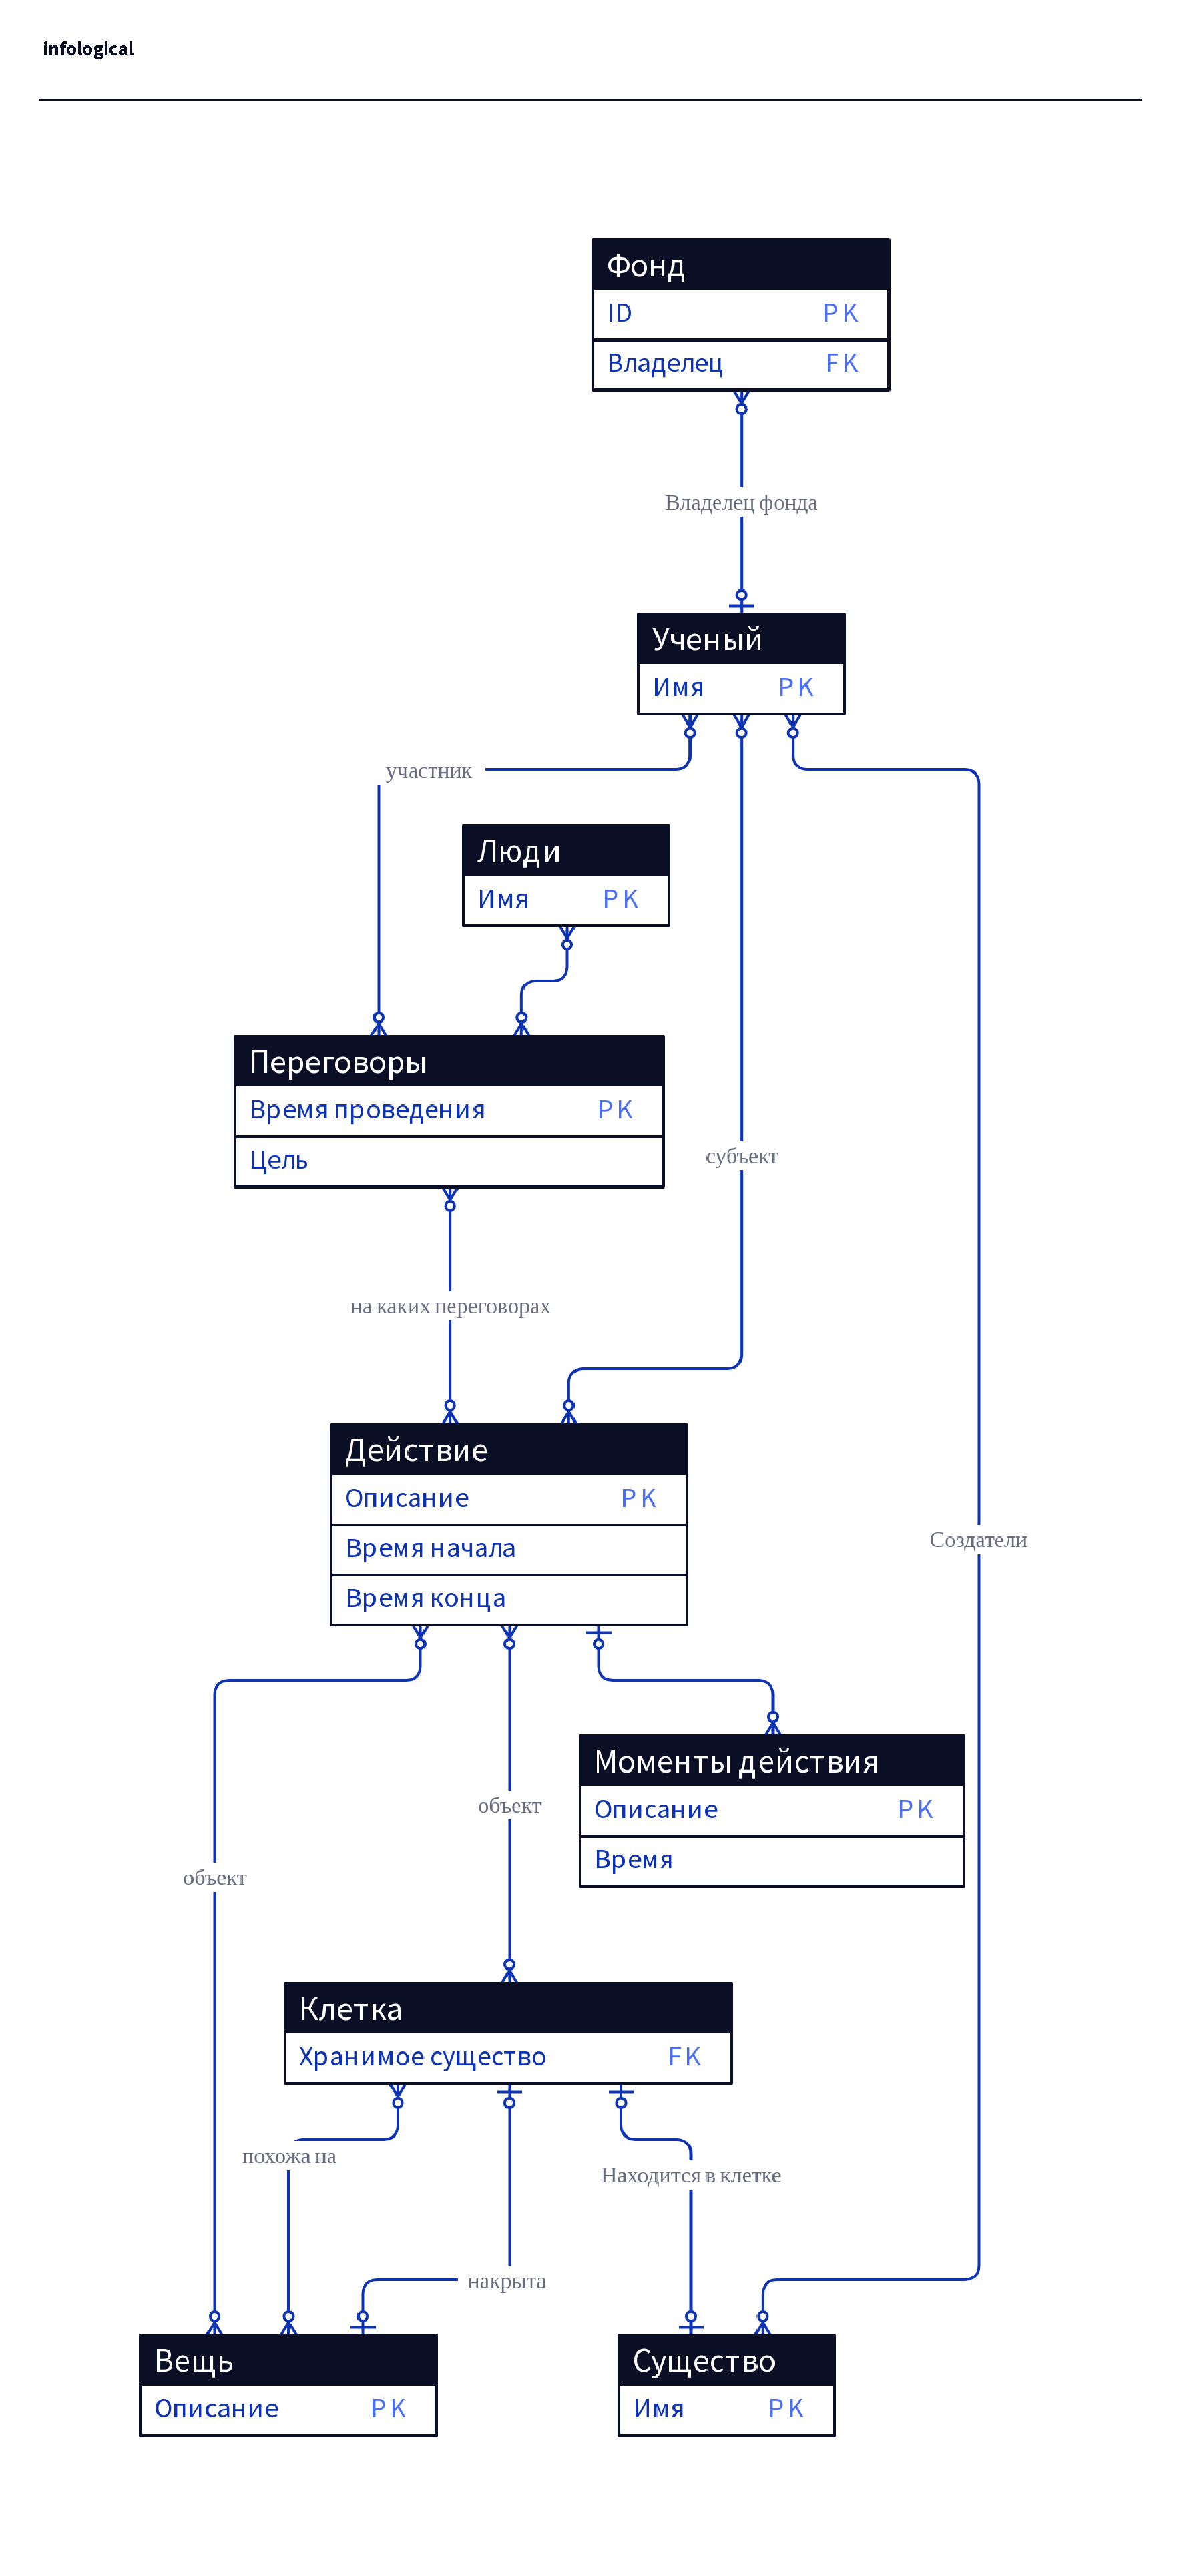
\includegraphics[height=0.4\textheight]{img/infological.pdf}
    \caption{Инфологическая модель}
\end{figure}


\begin{figure}[ht]
    \centering
    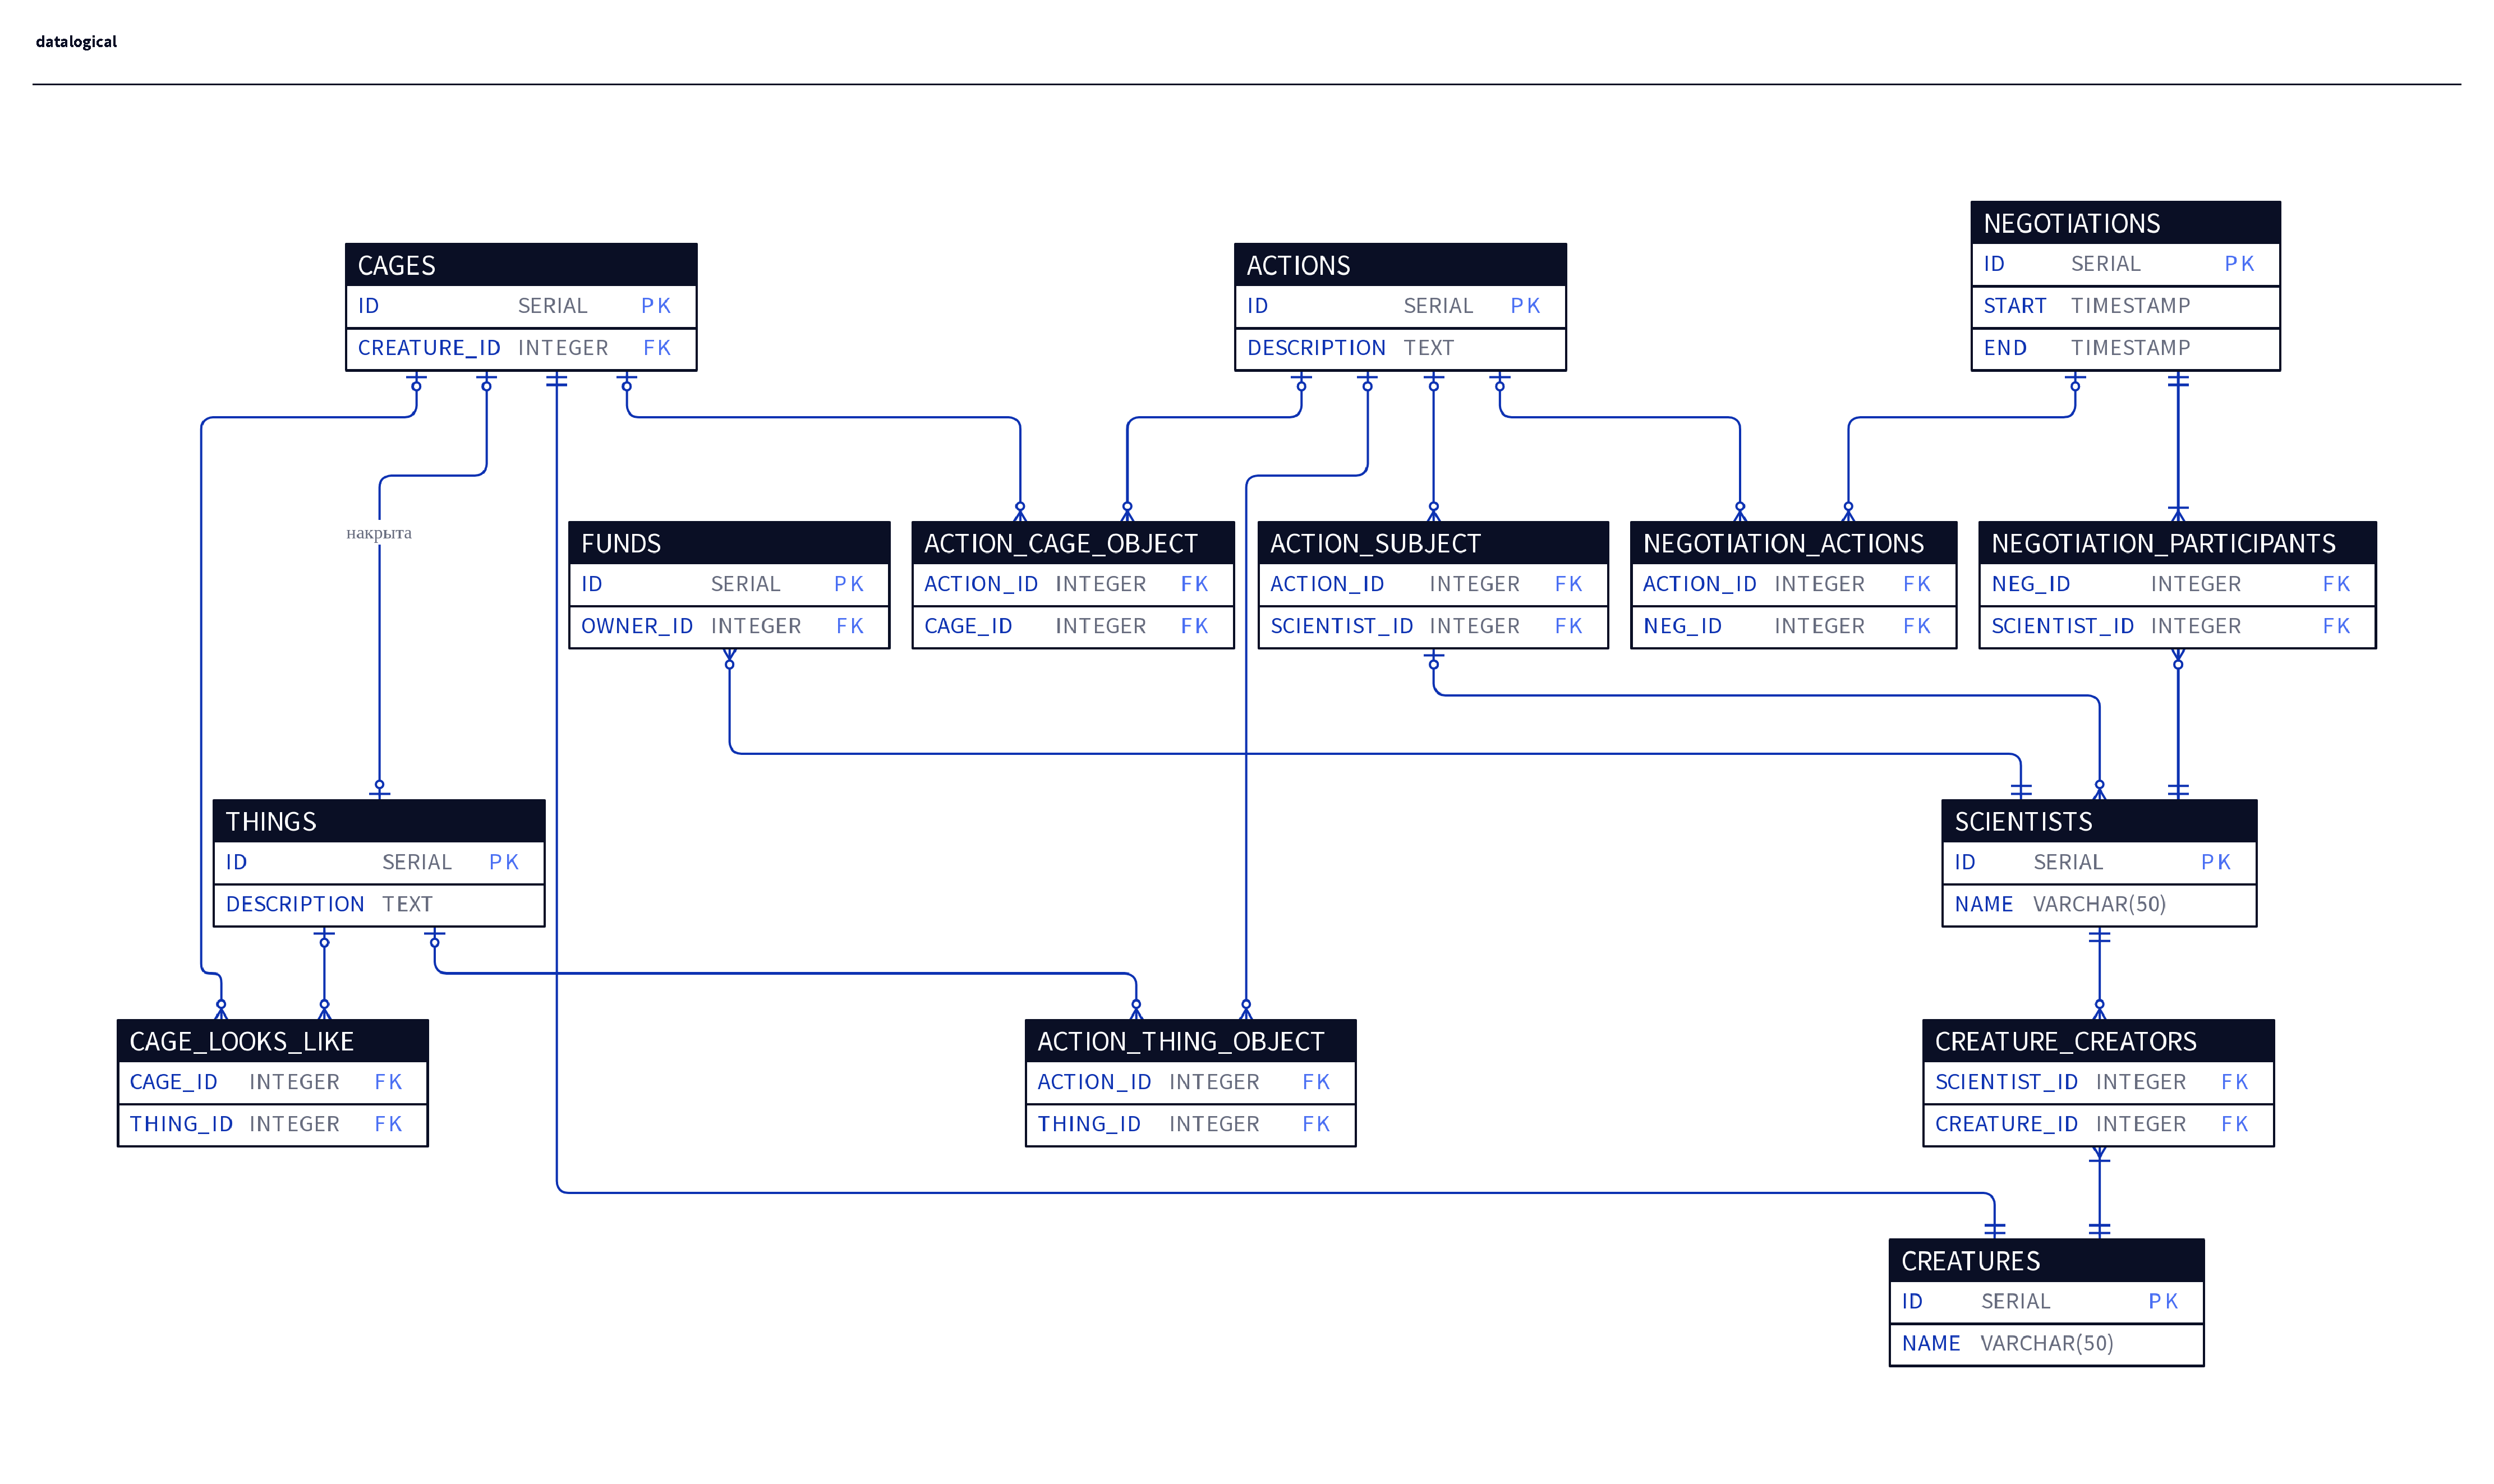
\includegraphics[width=\textwidth]{img/datalogical.pdf}
    \caption{Даталогическая модель}
\end{figure}

\subsection{Реализация модели на SQL}
\inputminted{SQL}{../scheme.sql}